\section{Background and Related Work}
\label{sec:related}

\subsection{Artificial Intelligence Techniques - Neural Networks}
\label{sub:aiml}
In this section we will describe common Artificial Intelligence (AI) techniques used in models for  facial expression recognition (Section \ref{sub:rw_fer}).
\subsubsection{Neural Networks}
A \emph{Neural Network NN} is built as a network with many \emph{neurons}, which are connected by \emph{activators} that have a \emph{weight}. These neurons are located in many layers which give structure to the NN \cite{schmidhuber2015deep}. The first layer of the NN is the so-called \emph{input layer}, which acts as the entry point for the data that is to be analysed. The last layer is defined as the \emph{output layer}. It contains the information about the estimation that the NN has made. The in-between layers are called \emph{hidden layers}.

More formally, each output of a neuron can be written as a function:

\begin{equation}
    h_i = \sigma (\sum_{j=1}^{N} w_{ij}x_{j})
\end{equation}

The function $\sigma$ describes the activation, $N$ the amount of neurons that are the input to the current neuron. The weight of the input connection from each neuron of the previous layer is described by $w$.

Activation functions can introduce non-linearity to a network. They can also bound the final value of an activation in a specific range to combat divergent neurons which may paralyze the NN \cite{wang2003artificial}. They also provide stability in gradient-based learning.
\bgroup
\def\arraystretch{2}
\begin{table}[]
    \centering
    \begin{tabular}{l|c|c}
        \textbf{Activation Function} & \textbf{Equation} & \textbf{Range} \\ \hline \hline
         Sigmoid & $\frac{1}{1 + e^{-x}}$ &  $(0,1)$\\\hline
         Softmax & $\frac{e^{x_i}}{\sum_{j=1}^{J} e^{x_i}}$ & $(0,1)$\\\hline
         ReLU & $max(0, x)$ & $[0, \infty]$ \\\hline
         Tanh & $\frac{e^x - e^{-x}}{e^x + e^{-x}}$ & $(-1, 1)$\\\hline
    \end{tabular}
    \caption{An overview of selected activation functions which we will use in our models (Section \ref{sec:models})}
    \label{tab:my_label}
\end{table}
\egroup

A NN can also be represented as a very complex function $f(x) = y$, where $x$ represents the input, and $y$ the computed output (the prediction).

Shallow NN consist of few hidden layers, and have been a topic for a long time. The discovery of \emph{backpropagation} allowed the development of NNs with many hidden layers, called \emph{Deep Neural Networks DNN} \cite{schmidhuber2015deep}.

\subsubsection{Convolutional Neural Networks CNN}
CNNs lend themselves well to tasks in \emph{Computer Vision CV} \cite{albawi2017understanding}. Most importantly, they reduce the amount of parameters, while also emphasizing locality and context of the input information. This enables edge detection, shape detection, and object detection in successive layers of a deep CNN, which will be especially helpful in models (Section \ref{sec:models}) that analyse faces and their active Action Units (Section \ref{subsub:au}).

Subsequent convolutional layers, coupled with pooling layers, enable the detection of more and more complex structures. While the initial layers might detect straight edges, the following layers will recognize compound structures, and ultimately features like raised eyebrows (AU 1 and/or AU 2).

\paragraph{Convolution}
The convolutional layers in a CNN provide locality and size reduction to the network. Since we work with image inputs in our thesis, we will provide such an example here.

Consider a greyscale image of a face with a width and height of 256x256 pixels. Each pixel is represented by a single greyscale value, putting the dimensionality of the image at 256x256x1. Layering this input image with a traditional dense layer of size 10 would already produce $256 \cdot 256 \cdot 10 = 655360$ weights that have to be trained. 

A (in this case two dimensional) convolutional layer only looks in local regions of the image to produce an output to the next layer. A sliding window of $n$ x $m$ pixels will scan the input image in a set stride, and produce values for the next layer with substantially less weights attached. Pre-set windows (also called matrices) of size 3 x 3 can be used to detect edges in images, or transform them with sharpening or blurring effects.

\paragraph{Pooling}
Pooling layers are used to decrease the size of the layers and create a more efficient embedding. A window of size $n$ x $m$ slides across the layer again, this time only producing a single value for each step. A common technique is to select the largest value in the current window, creating a so-called \emph{MaxPooling} layer. Figure \ref{fig:pooling} shows a MaxPooling layer working on a 4 x 4 matrix.

\begin{figure}
    \centering
    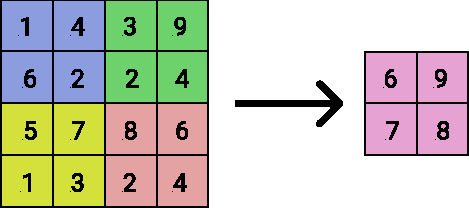
\includegraphics{res/pooling.pdf}
    \caption{An example of a MaxPooling layer working on the left matrix with a window size of 2 x 2 and a stride of 2, producing the matrix on the right.}
    \label{fig:pooling}
\end{figure}

\subsubsection{Temporal Neural Networks with Gated Recurrent Units GRU}
The previously described NNs can be described as \emph{feedforward} NNs. The direction of information flow is linearly through input, hidden and to the output layer. This can be contrasted with \emph{feedback} NNs, that have mechanisms that allow for 'memory' in a NN \cite{wang2003artificial}. These \emph{Recurrent Neural Networks RNN} enable the analysis of temporal data.

A concrete implementation for a temporal recurrent layer are \emph{Gated Recurrent Units GRU} proposed by Cho et al. \cite{cho2014properties} \cite{chung2014empirical}. GRUs act similarly to \emph{Long Short Term Memory LSTM} \cite{hochreiter1997lstm} layers, while removing memory gates \cite{chung2014empirical}. Empirical research has shown that GRUs can be more performant than LSTMs in less frequent datasets \cite{gruber2020gru}.


\subsubsection{Architectures}
NNs can be built in various different ways. Over time, researchers have developed predifined structures of NNs which are reused for many different applicaitons. These different structures are more commonly referred to as \emph{architecutres}. In this thesis we will come across the two well known architectures \emph{VGG} and \emph{MobileNet}.
\paragraph{VGG}
Introduced by Simonyan and Zisserman in 2014 \cite{simonyan2015vgg}, VGG16 and VGG19 have established themselves as architectures for image classification, including facial expression recognition. VGG16 achieved top-5 finishes in the 2014 ImageNet Challenge in both localisation and classification tasks. A major drawback to models using the VGG architecture is its computing performance. Given its rather large architecture, it is comparatively slow to train. This is where we turn to \emph{MobileNets}.
\paragraph{MobileNet}
\emph{MobileNets} were originally introduced for mobile and embedded vision applications \cite{howard2017mobilenets}. They allow for hyperparameter tuning, where the developer is able to choose a fitting model size for his application based on two global hyperparameters. MobileNets trade off accuracy (and thus the need for many hidden layers) in favour of speed and efficiency. Our core facial expression recognition models are based on the MobileNet architecture.


\subsection{Emotional Models from Facial Expression}
\label{sub:rw_fer}
We now need a way to leverage the tools we mentioned above to build models that accurately estimate the affective state. Ekman, Russell, Posner and many others have developed systems that rigidly define the emotional state of a subject. While dimensional models, which define the affective state through several dimensions, we will focus on the \emph{categorical model} that works on emotional classes. 

\paragraph{Categorical Model}
One of the most recognized ways to separate emotional states in non-verbal communication is presented by Paul Ekman \cite{ekman1987universals} \cite{ekman2013emotion}. His research postulates a cross-cultural agreement in judging facial expressions \cite{ekman1987universals}. Basic emotion theory assumes a fixed amount of human emotions, which is also believed and postulated by Ekman and Russell \cite{ekman1992basic} \cite{russell2006}. Ekman proposes a split into seven categories: anger, happiness, surprise, sadness, fear, disgust and contempt. He later consolidated them down to six, removing contempt. 

% \subsubsection{Dimensional Model}

% Dimensional systems use a set of dimensions, \emph{valence}, \emph{arousal} and in some cases \emph{dominance} to estimate the affective state of a person. James A. Russell introduced the two dimensional circumplex model of affect \cite{russell1980circumplex}, where he mapped emotions in the valence-arousal space. Valence represents the (un-)pleasantness of an affective state, and arousal represents the activation. \cite{posner2005circumplex}. The emotions from the categorical have their place in this dimensional field, e.g. happy having a high score for valence and arousal.

% \begin{figure}
%     \centering
%     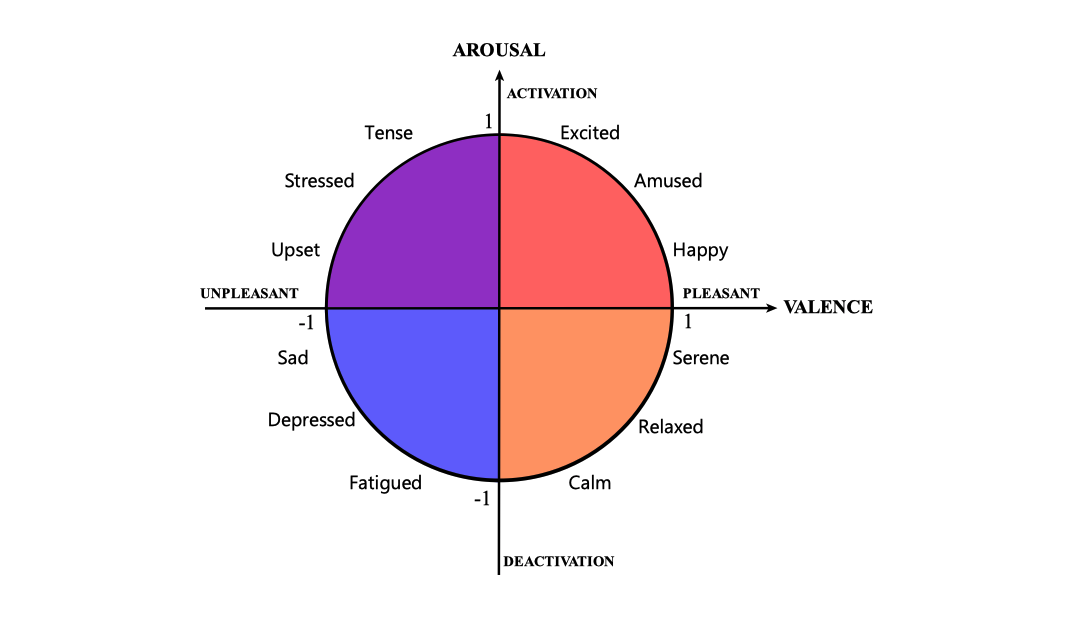
\includegraphics[width=0.8\textwidth]{res/circumplex.png}
%     \caption{The circumplex model of affect with the valence and arousal axis with selected emotions. \cite{russell1980circumplex} \cite{pourmirzaei2021an}}
%     \label{fig:circumplexImg}
% \end{figure}

\subsubsection{Action Units}
\label{subsub:au}

Introduced by Hjortsjö \cite{hjortsjo1969man} and further refined by Ekman \cite{friesen1978facial}, the \emph{Facial Action Coding System FACS} tries to separate and classify facial movements that lead to distinct facial expressions. Combinations of the 28 \emph{Action Units AUs} can then be used to describe an affective expression.

\begin{table}[]
    \centering
    \begin{tabular}{c|c}
       \textbf{Emotion}  & \textbf{Action Units} \\ \hline
        Happy & 12, 25 \\
        Sad & 4, 15 \\
        Fearful & 1, 4, 20, 25 \\
        Angry & 4, 7, 24 \\
        Surprised & 1, 2, 25, 26 \\
        Disgusted & 9, 10, 17
    \end{tabular}
    \caption{The basic emotions with their corresponding prototypical AUs \cite{fabian2016emotionet}}
    \label{tab:emotionAUs}
\end{table}

\subsection{Automatic Facial Emotion Recognition}
Facial Emotion Recognition FER can be divided into two different groups: conventional and Deep-Learning-based. \cite{ko2018brief}

Conventional FER systems work in a pipeline that consists of three steps: face detection, feature extraction and expression classification. The first step crops the input image to the face to ignore unneccesary input information. Facial landmarks can at times also be detected here. The second step detects features based on the data extracted from the previous step. Those features then are used to classify an emotion for the input \cite{ko2018brief}.

The deep learning approach has established itself as the state-of-the-art method for FER models. In contrast to the handcrafted conventional pipeline, the more modern approach enables an end-to-end learning method \cite{ko2018brief}. The most prominent model-type in FER is the convolutional neural network CNN. CNN-based networks offer themselves very well to image processing, which make them a great candidate for FER systems. 

Deep learning models can further be divided into two categories. The first one outputs emotions directly from the model \cite{ebrahimi2015recurrent} \cite{kim2017multi} \cite{jung2015joint}, where the second one classifies AU activations, from which emotions can be deduced \cite{breuer2017deep} \cite{zhao2016deep} \cite{chu2017learning}. 

\begin{figure}
    \centering
    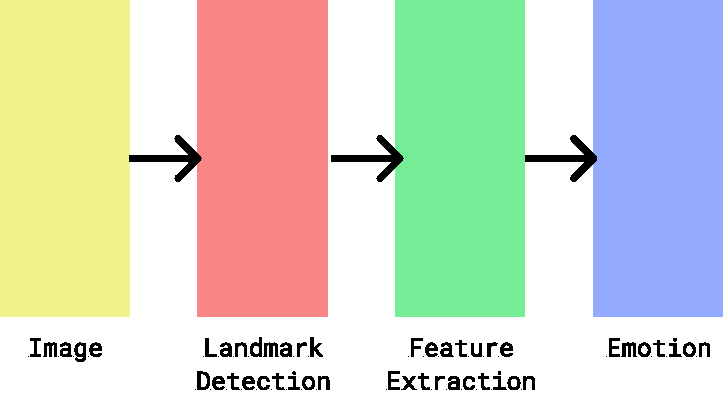
\includegraphics[width=0.8\textwidth]{res/PipelinePrototype.pdf}
    \caption{PROTOTYPE: An example of a FER pipeline. After extracting landmarks from the target image, models try to extract features from the given landmarks. These can be used to detect an emotion from the input.}
    \label{fig:pipeline_fer}
\end{figure}

\subsection{Phonemes and Visemes}
The content of an act of speech can be segmented into words, syllables, and \emph{phonemes} \cite{savin1970nonperceptual}. Languages differ in their amount of phonemes, with the New Guinean language Rotokas having 11, whereas the Namibias !Xóõ is using 160. English, the primary language we're be looking at in this thesis, has 37-41 phonemes, differing by dialect \cite{Hayes2009}. Phonemes are very important in FER. A speaking subjects face, and activated AUs, will be influenced by the lexical content of their speech, which is defined by the current phoneme. The face of a person in the act of pronouncing a phoneme will have a certain look to it. Several phonemes can be grouped together based on the distinct look they produce. These groups are called \emph{visemes}. There are several different phoneme-to-viseme mappings in research, with no concrete agreement on a 'best mapping' \cite{cappelletta2012viseme}.

Visemes are particularly interesting for us, since our research is purely based in the visual domain. Differences between phonemes that are purely audiocentric are of no relevance for us. A viseme mapping reduces the categories for visually based lexical content, which makes building and training models easier.

\begin{figure}
    \centering
    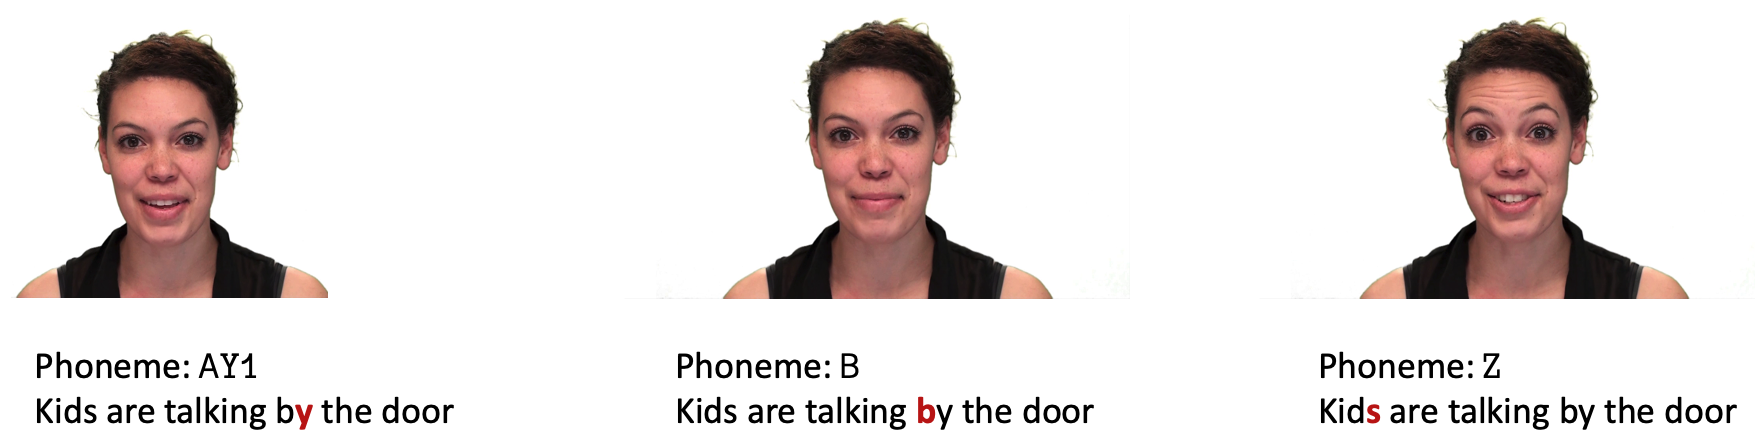
\includegraphics[width=0.8\textwidth]{res/phoneme.png}
    \caption{A visual example of three phonemes being spoken, together with their occurrence in a sentence.}
    \label{fig:phoneme_ex}
\end{figure}

\subsubsection{LipNet}

LipNet is an end-to-end sentence-level lipreading model that is based on visual data \cite{assael2016lipnet}. It specifically is not based on word classification, the authors stress the sentence-level lipreading comprehension. It operates on the character-level, combining CNNs with RNNs.

\begin{figure}
    \centering
    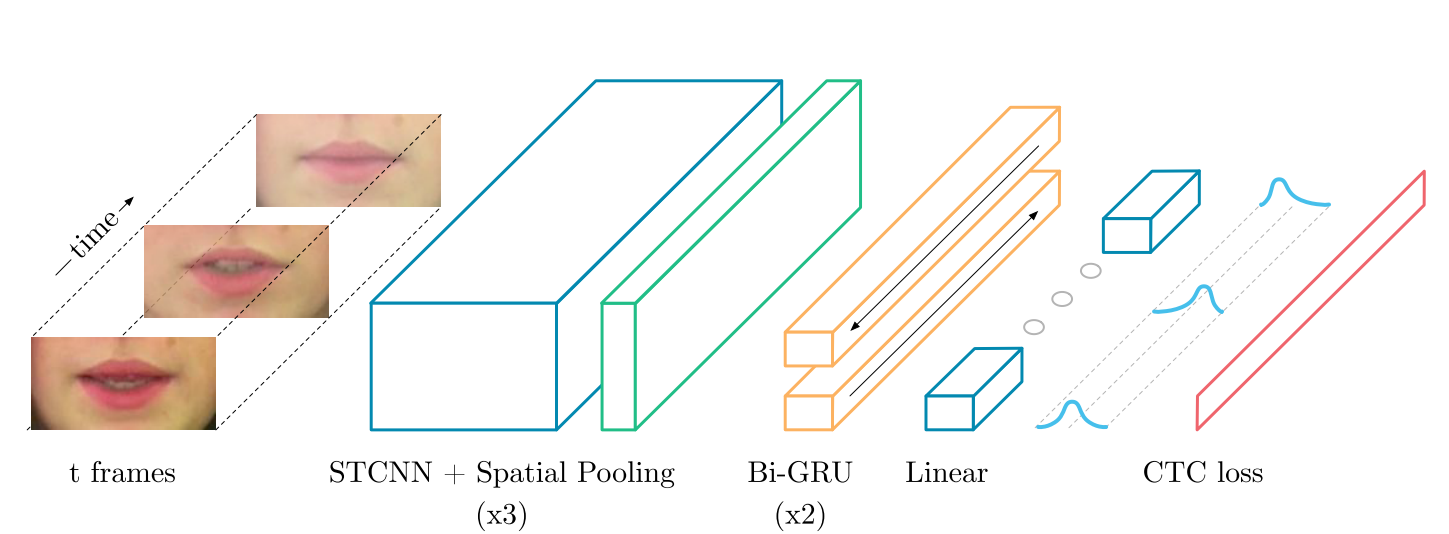
\includegraphics[width=0.8\textwidth]{res/lipnet.png}
    \caption{The architecture of LipNet \cite{assael2016lipnet}. A batch of \textit{t} frames is fed into the network. A combination of Spatio-Temporal CNN layers with Spatial Pooling layers feed into two GRUs.}
    \label{fig:lipnet}
\end{figure}

The LipNet model is trained on the GRID corpus \cite{cooke2006grid}, where it achieves a 95.2\% sentence-level word accuracy.

The input of the model is a cropped region around the orofacial area of the face. The dimension of this region is set to 100x50 pixels, and the default frame batch size is set to 75 frames.

We will use an embedding of LipNet in one of our models to create a lexical compensator.

\subsubsection{FaceMesh}


FaceMesh is a model to create 3-dimensional models of the facial surface geometry in real time videos \cite{kartynnik2019facemesh}. It creates 468 3-dimensional landmark points on the face, which are arranged in fixed quads.

\begin{figure}
    \centering
    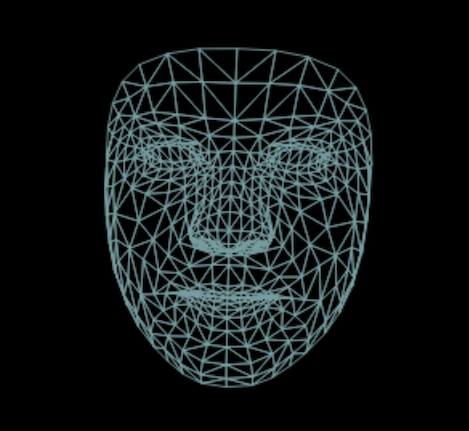
\includegraphics[width=0.5\textwidth]{res/facemesh2.png}
    \caption{The mesh topology of FaceMesh. The 468 landmark points are projected on a screen. Neighbouring points are connected to form three-sided polygons.}
    \label{fig:facemesh}
\end{figure}

FaceMesh was originally implemented in tensorflow.js, making it only available on JavaScript runtimes. The mediapipe project published a port to a Python implementation, which we used of our models.

The model was trained on around 30,000 diverse, in-the-wild images which were also augmented while training. Annotating the images was done in an iterative approach \cite{kartynnik2019facemesh}:
\begin{enumerate}
    \item Initial model in supervised approach through synthetic renderings of 3D morphable models or 2D landmarks from annotated in-the-wild images.
    \item Refine the x- and y-coordinates by using the latest model while filtering out predictions where the prediction error is tolerable. Other predictions were improved through annotation.
\end{enumerate}
\subsubsection{Montreal Forced Aligner}
\label{sub:mfa}
The Montreal Forced Aligner MFA is an open source software for speech-text alignment \cite{mcauliffe2017montreal}. A forced aligner is a tool that aligns speech and it's corresponding transcription on a word and phone level. This allows for precise estimations of phoneme occurrence in audio files.

The MFA builds on Kaldi \cite{povey2011kaldi}, a speech recognition toolkit which allows for easy distribution due to Kaldi's open-source license.

We will use the MFA to align our datasets and to get a precise phoneme-to-video mapping, enabling us to extract frames where specific phonemes were said by the actors.

\begin{figure}
    \centering
    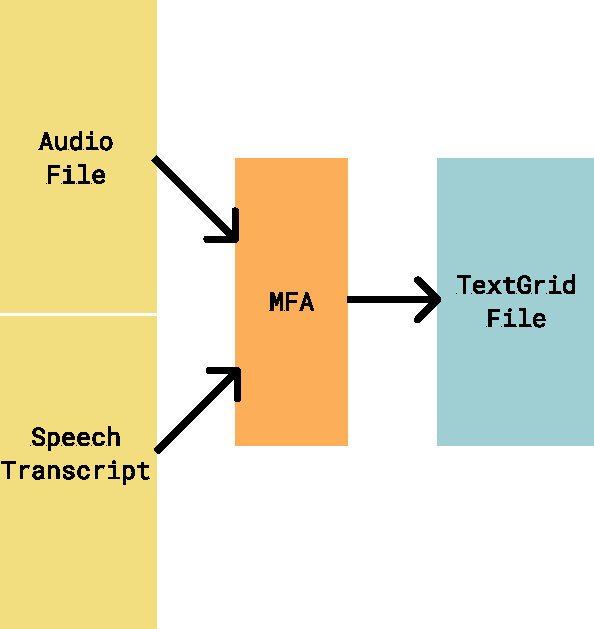
\includegraphics[width=0.5\textwidth]{res/mfa.pdf}
    \caption{A pipeline of a classic use of the MFA. An audio file, together with its transcript gets fed into the MFA. The output of the aligner is a \texttt{TextGrid} file that contains timestamp information about word and phoneme occurrence in the input audio file.}
    \label{fig:mfa}
\end{figure}
\subsection{Existing Approaches to Compensate Speech Effects}
\label{sec:existing}
There have already been advances in FER that accounts for speech. In this section, we will present three models that will be relevant to our work.

\subsubsection{Blind Lexical Compensation}
Mariooryad and Busso \cite{mariooryad2015facial} propose a model that bases itself on a previous study, stating that facial expressions are the result of three factors that influence facial behaviours:

\begin{enumerate}
    \item The individual features and habits of the speaker
    \item The lexical content of the speech act
    \item The current affective state/emotion of the subject
\end{enumerate}

Their analysis also showed that "constraining the model on the lexical content makes the emotion variability the dominant factor in the mouth area" \cite{mariooryad2015facial} \cite{mariooryad2012factorizing}.

The authors aim to build a model using blind lexical compensation, a method that will not require a transcription of the lexical content. Their approach builds on the asymmetric bilinear model \cite{tenenbaum1997separating} \cite{tenenbaum2000separating}. This model aims to separate style from content. In this case, the style represents the emotion and the individual phoneme the content.

After training, the model consists of $N$ style matrices (with $N$ being the amount of emotions). Each style matrix represents an embedding for the corresponding emotion. To classify an input sample, the \emph{Expectation Maximization EM} algorithm was used, to achieve a soft assignment $p(s^{*}, c |y)$ (the probability of the sample $y$ belonging to style $s^{*}$ and content $c$.

After 10 EM cycles, a style matrix $A^{*}$ will be produced. The emotion estimation is done by calculating the frobenius norms to each trained style matrix, and using the label of the style matrix with the lowest distance.

Given that this approach requires facial landmarks and artificial mesh alrorithms were not as established at the time, the dataset of choice was IEMOCAP. This leads to the model only having four classes (Happiness, Anger, Sadness, Neutrality).

\subsubsection{Lexical Compensation with LipNet}
Bursic et al. \cite{bursic2020improving} created a NN centered around lexical compensation using LipNet. While they present several approaches in their paper, we are most interested in their Lip Model, which is build by merging a LipNet embedding with an embedding of a classic VGG19 FER model. The models have also been temporalized, with several different frame batches ranging from 5 to 65 frames. Their best performing Lip Model was set at 60 frames per prediction, reaching an accuracy of 59.4\%. In comparison, the face-only RNN model that does not include lexical compensation from LipNet reached it's best accuracy at 40 frames and 48.5\%.

The dataset used in this paper was RAVDESS, using the core emotions from Ekman, ignoring \emph{calm}. This makes for a good comparison to our models.

We will compare our experiments of using LipNet as a lexical compensator their results in section \ref{sec:models}.

\begin{figure}
    \centering
    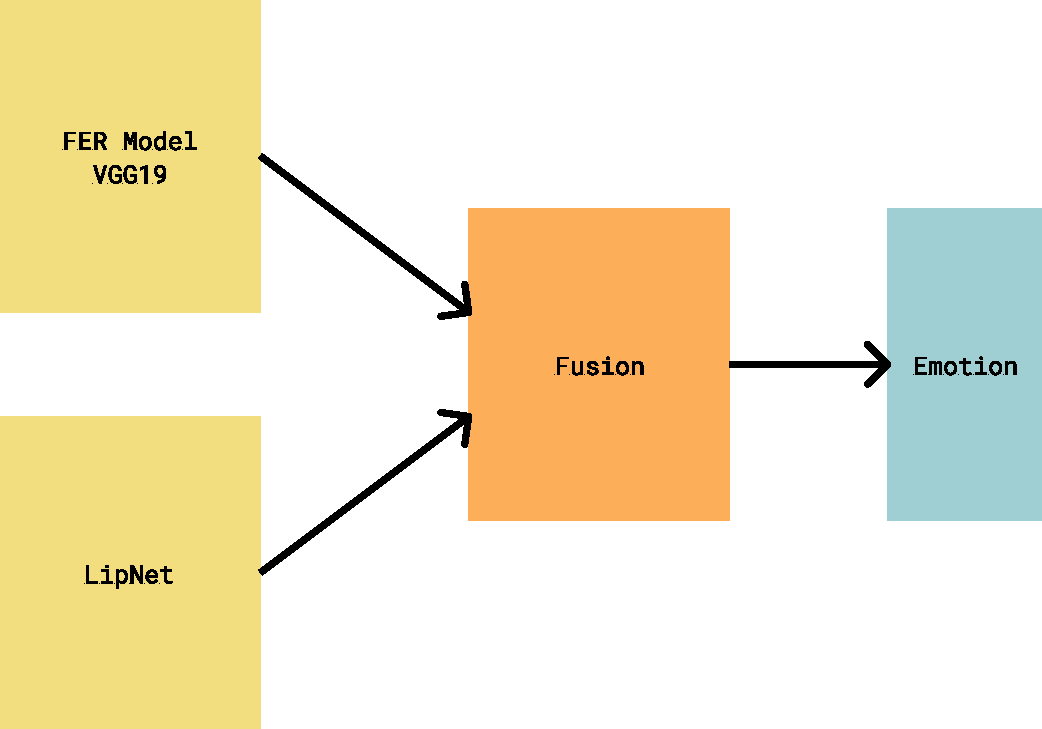
\includegraphics[width=0.8\textwidth]{res/bursicschema.pdf}
    \caption{The schema of the Lip RNN by Bursic et al. \cite{bursic2020improving}.}
    \label{fig:bursic_schema}
\end{figure}

\subsubsection{Lexical Compensation using a Style Extractor}
Salman and Busso \cite{salman2020style} have a similar approach to Bursic, using a lexical compensator alongside a feature extractor with an embedding of a classic FER model using the VGG16 architecture.

The major point of interest is their style extractor/lexical compensator (see Figure \ref{fig:bussose}). It uses facial meshes of the subject instead of images, generalizing it against the subject. The model is trained on a temporal NN with one input and two outputs: an emotional mesh of a face serves as the input, producing a neutral mesh alongside a phoneme prediction. The idea is that the difference between the emotional input mesh and the neutral output mesh can give us information about the facial movements that are produced by emotional activations.

We will use a similar feature extractor in our experiments. Since Salman and Busso only trained their model on four emotions, comparisons will be challenging. We will rather compare our results with the performance of our other models, trying to determine the impact of the lexical compensator that way. 

\begin{figure}
    \centering
    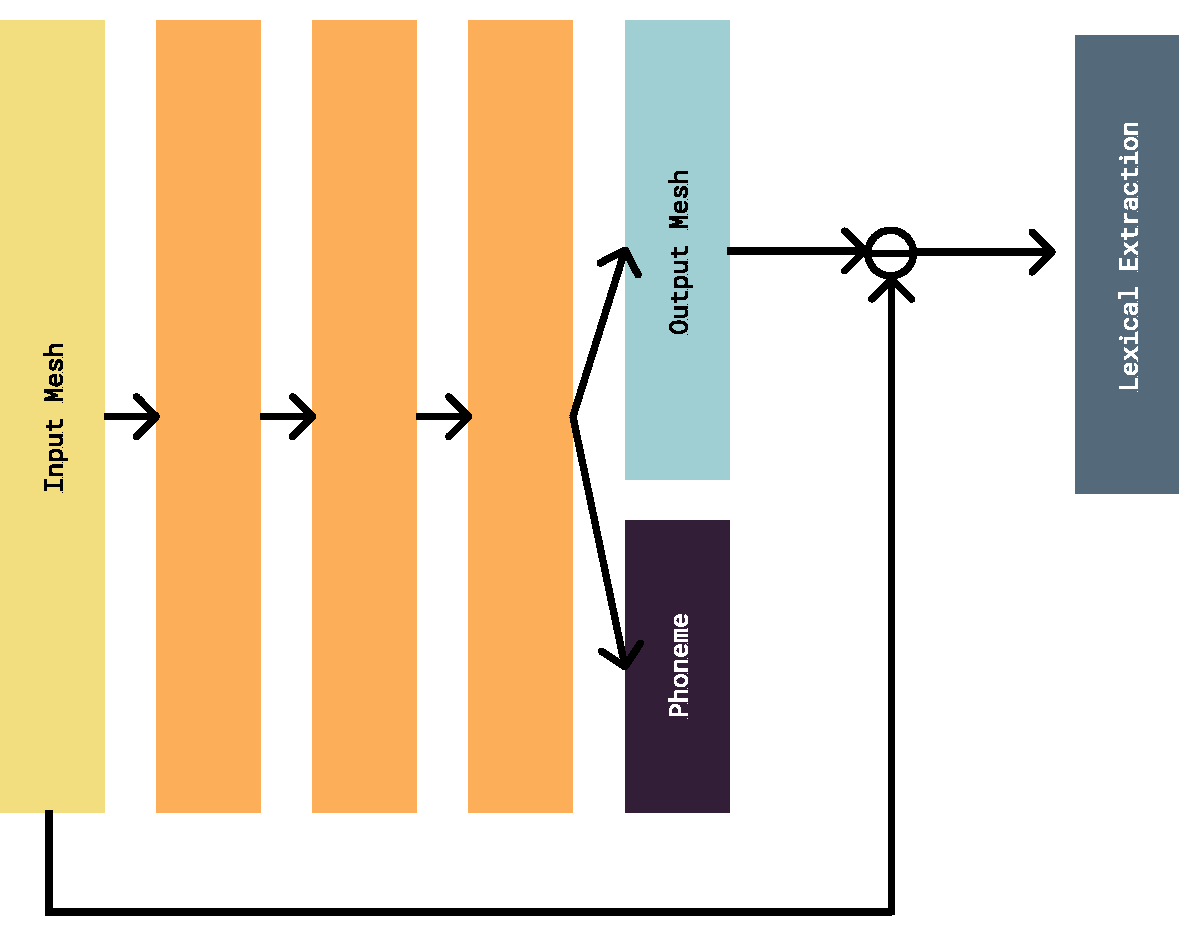
\includegraphics[width=0.8\textwidth]{res/BussoSE.pdf}
    \caption{The schemal of Salman and Busso's lexical compensator. An emotional mesh is the input to a NN, producing a neutral output mesh alongside a phoneme prediction. The difference of the input mesh and the output mesh extracts the facial movements that are produced by the emotional state of the subject.}
    \label{fig:bussose}
\end{figure}

\subsubsection{Temporal Compensation}
The previous two models both used a temporal approach alongside their efforts of lexical compensation. Opposed to the more traditional way of FER where only single images were classified, a temporal model estimates the emotion on a sequence of images. 


\subsection{Datasets}

\subsubsection{AffectNet}
\emph{AffectNet} is one of the largest image databases for affect. It consists of around 450,000 manually annotated images. Labellers classified them by eight emotional categories (Neutral, Happy, Sad, Surprise, Fear, Anger, Disgust, Contempt) while also providing continuous labels for valence and arousal. In addition to the labelled images, 1,000,000 images with facial landmarks are provided.

The images were collected by scraping the internet through querying various search engines. Faces were recognized with the \emph{OpenCV} toolkit. Facial landmarks were extracted with regression of binary features \cite{ren2014face}.

Labelling the 450,000 images was done by 12 full-time and part-time annotators who were knowledgeable on the issues of emotion and affect, and were specifically hired for the task. This was done to remove the issue of low-quality labels that occur with crowd-sourced methods. \cite{mollahosseini2017affectnet}

Our classic FER models we will use are all trained on AffectNet.

\subsubsection{RAVDESS}
\label{sub:ravdess}
The Ryerson Audio-Visual Database of Emotional Speech and Song (RAVDESS) is a validated multimodal database for emotional analysis \cite{livingstone2018ryerson}. It contains videos of speech and song from 24 professional actors. The database is gender balanced, and the actors were chosen with the ability of speaking a neutral North American accent. The database contains videos in eight emotions (Calm, Happy, Sad, Angry, Fearful, Surprise, Disgust, Neutral) in the speech acts, which are the important ones for us.

The actors were tasked with speaking two pre-defined sentences ("Dogs are sitting by the door", "Kids are talking by the door") in the given emotions, across two levels of intensity. Across all actors, 1440 audio-visual files of speech acts were recorded. Audio- and video-only files are provided as well.

RAVDESS lends itself very well to our research by including all core emotions and providing high quality footage. It also standardizes statements and lexical content, which lowers the amount of external factors that could influence our analysis and training. We focus our attention to the core emotions that are described by Ekman, which means that we ignored the videos for the calm emotion.

\begin{figure}
    \centering
    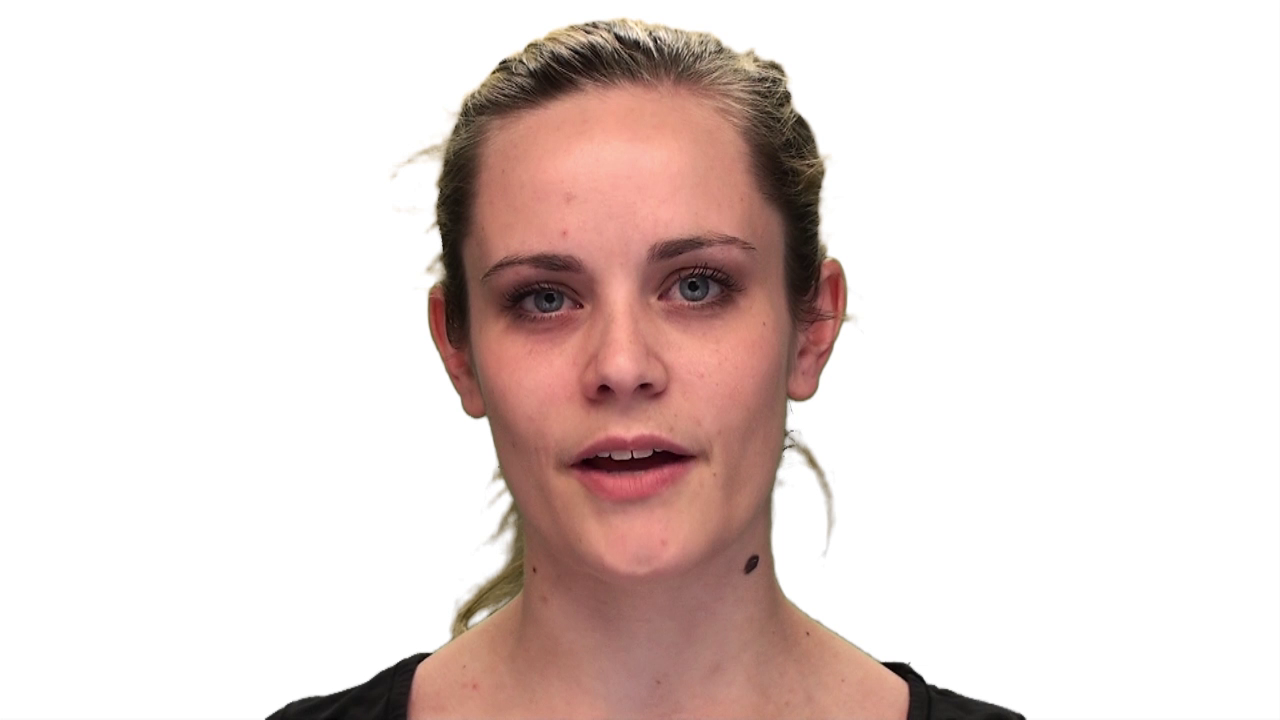
\includegraphics[width=0.8\textwidth]{res/img_ravdess_example_neutral_14AY1.png}
    \caption{A frame of a video from the RAVDESS database \cite{livingstone2018ryerson}. Actor 14 is pronouncing the phoneme \texttt{AY1} in a neutral emotion.}
    \label{fig:ravdess_example}
\end{figure}

\subsubsection{CREMA-D}
The Crowd-sourced Emotional Multi-modal Actors Database (CREMA-D) is a labelled multimodal for emotional analysis \cite{cao2014crema}. It contains 7,442 videos of speech acts from 91 actors of varying age and ethnicity. The database includes videos across seven emotions (Calm, Happy, Sad, Angry, Fearful, Disgust, Neutral) with scaled intensities. Surprised is notably missing from the emotional categories. The authors state that "surprise was not considered by the acting directors to be sufficiently specific, as it could relate to any of the other emotions with rapid onset" \cite{cao2014crema}. 

The authors also provided the individual ratings for each video, which were collected from 2,443 crowd-sourced raters. These can also be used to analyse human bias in emotion recognition (see Section \ref{sec:human}).

\subsubsection{MSP-IMPROV}
MSP-IMPROV is an acted multimodal database for emotional analysis \cite{busso2016msp}. It covers four emotions (Anger, Happiness, Sadness, Neutral), where twelce actors (6 male, 6 female) were tasked to speak 15 different statements. While recording, the actors were set in different scenarios, in which the target sentences were included. Only the target sentence had to be spoken word-for-word, the buildup to the scenario was open to improvisation.

652 recordings are provided on the target sentences. The authors also provide the statements on the entire improvised session, where 4,381 speaking turns are collected. 2,785 speaking turns were collected on natural interactions, where the actors were speaking normally to each other, outside of a scripted or improvised session. 620 turns were recorded on the target sentences alone, where the actors were tasked to read the statements in the provided emotion. This sums up the size of the MSP-IMPROV corpus to 7,818 recordings. 

\subsubsection{IEMOCAP}
The interactive emotional dyadic motion capture database (IEMOCAP) \cite{busso2008iemocap} is a labelled database based on dyadic interaction where one of the subjects is set up with motion capture software on their head, face and wrists. It is based on two types of interactions, acted and improvised.

The database is gender balanced, with 5 male and female actors each. The actors were students from the Drama Department of the University of Southern California.

The data was annotated by USC students. They labelled the utterances based on categorical expression (Neutral, Happiness, Sadness, Anger, Surprise, Fear, Disgust, Frustration, Excited, Other) and dimensional values for activation, valence, and dominance.

In total, 5,255 scripted turns and 4,784 improvised turns were recorded. 

\begin{figure}
    \centering
    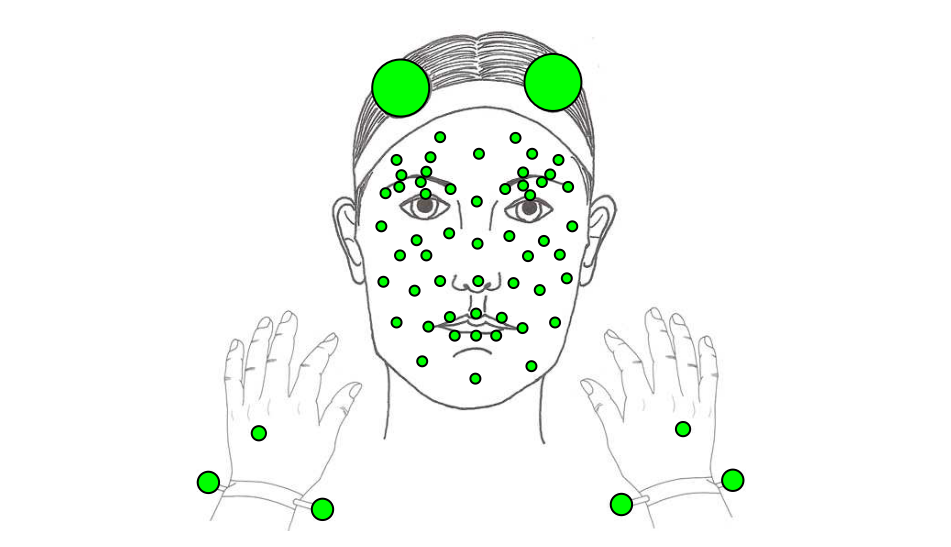
\includegraphics[width=0.8\textwidth]{res/iemocap.png}
    \caption{The motion capture points of IEMOCAP. They cover 53 points on the face, a wristband with two markers, one marker for each hand, and a headband with two markers. \cite{busso2008iemocap}}
    \label{fig:iemocap_cap}
\end{figure}
